\documentclass{templateNote}
\usepackage{amssymb}
\usepackage{pgfplots}

\pgfplotsset{compat=1.18}

\definecolor{Verde}{RGB}{170,239,31}
\definecolor{Morado}{RGB}{127,0,255}
\definecolor{Celeste}{RGB}{0,191,255}
\definecolor{Salmon}{RGB}{255,0,157}

\newcolumntype{g}{>{\columncolor{green!50}}c}
\begin{document}

\imagenlogoU{img/LogoElNube.png}
\linklogoU{https://github.com/MarceloPazPezo}
\linkQRDoc{https://github.com/MarceloPazPezo/MyRepo/blob/main/Icinf/Semestre\%207/Investigaci\%C3\%B3n\%20de\%20Operaciones/Formativa\%201/Formativa-1.pdf}
\titulo{Formativa 1 (Certamen 1 ICI)}
\asignatura{Investigación de Operaciones}
\autor{
Marcelo Paz
}
\vDoc{1.3.2}

% Metadatos del PDF
\title{[\asignatura]-\titulo}
\author{
    \autor
}
\portada
\margenes % Crear márgenes

\section*{Problema 1}

La empresa MADERAS C. A. es un fabricante de muebles. Hace tres estilos diferentes de
mesas, A, B, C. Cada modelo de mesa requiere de una cierta cantidad de tiempo para el corte
de las piezas, su montaje y pintura. MADERAS C.A., puede vender todas las unidades que
fabrica. Es m\'as, el modelo B se puede vender sin pintar. Utilizando los datos indicados,
obtener el modelo lineal que permita determinar la m\'axima utilidad mensual que puede
obtener la Empresa.
\begin{figure}[H]
    \centering
    \begin{tabular}{|l|c|c|c|c|}
        \hline
        \multicolumn{5}{|r|}{Requerimiento de Horas Hombre por mesa} \\ \hline
        Modelo & Utilidad por mesa & Corte & Ensamblado & Pintura \\ \hline
        A & \$17.500 & 1 & 2 & 4 \\
        B & \$20.000 & 2 & 4 & 4 \\
        B sin pintar & \$10.000 & 2 & 4 & 0 \\
        C & \$25.000 & 3 & 7 & 5 \\ \hline
          & Disponibilidad mensual de HH & 200 & 298 & 148 \\ \hline
    \end{tabular}
\end{figure}

\subsection*{Declaraci\'on de variables:}
\begin{itemize}
    \item $x_1$: Cantidad de mesas A a fabricar.
    \item $x_2$: Cantidad de mesas B a fabricar.
    \item $x_3$: Cantidad de mesas B sin pintar a fabricar.
    \item $x_4$: Cantidad de mesas C a fabricar.
\end{itemize}

\subsection*{Función Objetivo:}
\begin{equation*}
    \begin{aligned}
        \text{Max} \quad & Z = 17500x_1 + 20000x_2 + 10000x_3 + 25000x_4 \\
        \text{s.a} \quad & x_1 + 2x_2 + 2x_3 + 3x_4 \leq 200 \\
        & 2x_1 + 4x_2 + 4x_3 + 7x_4 \leq 298 \\
        & 4x_1 + 4x_2 + 5x_4 \leq 148 \\
        & x_1, x_2, x_3, x_4 \geq 0
    \end{aligned}
\end{equation*}


\subsection*{Por método Simplex (Solo para practicar)}
\begin{itemize}
    \item \textbf{P.3:} Agregamos variables de holgura.
    \begin{equation*}
        \begin{aligned}
            & x_1 + 2x_2 + 2x_3 + 3x_4 + s_1 \leq 200 \\
            & 2x_1 + 4x_2 + 4x_3 + 7x_4 + s_2 \leq 298 \\
            & 4x_1 + 4x_2 + 5x_4 + s_3 \leq 148 \\
            & x_1, x_2, x_3, x_4, s_1, s_2, s_3 \geq 0
        \end{aligned}
    \end{equation*}

    \item \textbf{P.6:} Iguala las restricciones, y reescribimos la función objetivo.
    \begin{equation*}
        \begin{aligned}
            & x_1 + 2x_2 + 2x_3 + 3x_4 + s_1 = 200 \\
            & 2x_1 + 4x_2 + 4x_3 + 7x_4 + s_2 = 298 \\
            & 4x_1 + 4x_2 + 5x_4 + s_3 = 148 \\
            & x_1, x_2, x_3, x_4, s_1, s_2, s_3 \geq 0
        \end{aligned}
    \end{equation*}
    \begin{equation*}
        \therefore
    \end{equation*}
    \begin{equation*}
        \begin{aligned}
            \text{Max} \quad & Z = 17500x_1 + 20000x_2 + 10000x_3 + 25000x_4 \\
            \text{s.a} \quad & x_1 + 2x_2 + 2x_3 + 3x_4 + s_1 = 200 \\
            & 2x_1 + 4x_2 + 4x_3 + 7x_4 + s_2 = 298 \\
            & 4x_1 + 4x_2 + 5x_4 + s_3 = 148 \\
            & x_1, x_2, x_3, x_4, s_1, s_2, s_3 \geq 0
        \end{aligned}
    \end{equation*}

    \item \textbf{P.9:} Rellenamos la tabla simplex, con las ecuaciones.
    \begin{center}
        \begin{tabular}{|c|c|c|c|c|c|c|c|c|c|}
            \hline
            & & 17500 & 20000 & 10000 & 25000 & 0 & 0 & 0 & \\ \hline
            $C_j$ & \textbf{V.B} & $x_1$ & $x_2$ & $x_3$ & $x_4$ & $s_1$ & $s_2$ & $s_3$ & RHS \\ \hline
            0 & $s_1$ & 1 & 2 & 2 & 3 & 1 & 0 & 0 & 200 \\
            0 & $s_2$ & 2 & 4 & 4 & 7 & 0 & 1 & 0 & 298 \\
            0 & $s_3$ & 4 & 4 & 0 & 5 & 0 & 0 & 1 & 148 \\ \hline
            & $Z_j$ & & & & & & & & \\ \hline
            & $C_j - Z_j$ & & & & & & & & \\ \hline
        \end{tabular}
    \end{center}

    \item \textbf{P.10:} Calculamos $Z_j$.
    \begin{center}
        \begin{tabular}{|c|c|c|c|c|c|c|c|c|c|}
            \hline
            & & 17500 & 20000 & 10000 & 25000 & 0 & 0 & 0 & \\ \hline
            $C_j$ & \textbf{V.B} & $x_1$ & $x_2$ & $x_3$ & $x_4$ & $s_1$ & $s_2$ & $s_3$ & RHS \\ \hline
            0 & $s_1$ & 1 & 2 & 2 & 3 & 1 & 0 & 0 & 200 \\
            0 & $s_2$ & 2 & 4 & 4 & 7 & 0 & 1 & 0 & 298 \\
            0 & $s_3$ & 4 & 4 & 0 & 5 & 0 & 0 & 1 & 148 \\ \hline
            & $Z_j$ & 0 & 0 & 0 & 0 & 0 & 0 & 0 & $\underline{0}$ \\ \hline
            & $C_j - Z_j$ & & & & & & & & \\ \hline
        \end{tabular}
    \end{center}

    \newpage
    \item \textbf{P.11:} Calculamos $C_j - Z_j$.
    \begin{center}
        \begin{tabular}{|c|c|c|c|c|c|c|c|c|c|}
            \hline
            & & 17500 & 20000 & 10000 & 25000 & 0 & 0 & 0 & \\ \hline
            $C_j$ & \textbf{V.B} & $x_1$ & $x_2$ & $x_3$ & $x_4$ & $s_1$ & $s_2$ & $s_3$ & RHS \\ \hline
            0 & $s_1$ & 1 & 2 & 2 & 3 & 1 & 0 & 0 & 200 \\
            0 & $s_2$ & 2 & 4 & 4 & 7 & 0 & 1 & 0 & 298 \\
            0 & $s_3$ & 4 & 4 & 0 & 5 & 0 & 0 & 1 & 148 \\ \hline
            & $Z_j$ & 0 & 0 & 0 & 0 & 0 & 0 & 0 & $\underline{0}$ \\ \hline
            & $C_j - Z_j$ & 17500 & 20000 & 10000 & 25000 & 0 & 0 & 0 & \\ \hline
        \end{tabular}
    \end{center}

    \item \textbf{P.12:} Seleccionamos la variable de entrada.
    \begin{equation*}
        \colorbox{green!50}{$V_{in}$} = \text{columna Max} \{C_j-Z_j\} = X_{j^*} \Rightarrow V_{in} = x_4 : 25000
    \end{equation*}

    \item \textbf{P.13:} Calculamos el cociente mínimo y seleccionamos la variable de salida, para elegir el pivote.
    \begin{align*}
        s_1: \frac{200}{3} = 66.67 \qquad s_2: \frac{298}{7} = 42.57 \qquad s_3: \frac{148}{5} = 29.6 \\
    \end{align*}
    \begin{equation*}
        \colorbox{red!50}{$V_{out}$} = \text{Min} \left\{ \frac{RHS}{coef_{ij^*}} \right\} = i^* \Rightarrow V_{out} = s_3 : 29.6
    \end{equation*}
    \begin{center}
        \begin{tabular}{|c|c|c|c|c|g|c|c|c|c|}
            \hline
            & & 17500 & 20000 & 10000 & 25000 & 0 & 0 & 0 & \\ \hline
            $C_j$ & \textbf{V.B} & $x_1$ & $x_2$ & $x_3$ & $x_4$ & $s_1$ & $s_2$ & $s_3$ & RHS \\ \hline
            0 & $s_1$ & 1 & 2 & 2 & 3 & 1 & 0 & 0 & 200 \\
            0 & $s_2$ & 2 & 4 & 4 & 7 & 0 & 1 & 0 & 298 \\
            \rowcolor{red!50}0 & $s_3$ & 4 & 4 & 0 & 5 & 0 & 0 & 1 & 148 \\ \hline
            & $Z_j$ & 0 & 0 & 0 & 0 & 0 & 0 & 0 & $\underline{0}$ \\ \hline
            & $C_j - Z_j$ & 17500 & 20000 & 10000 & 25000 & 0 & 0 & 0 & \\ \hline
        \end{tabular}
    \end{center}
    \begin{center}
        $\text{Pivote} = a_{i^*j^*} = a_{34} = 5$
    \end{center}

    \item \textbf{P.14:} Calculamos la nueva tabla simplex.
    \begin{align*}
        x_4: \quad \textbf{N.E.P} = \frac{\textbf{E.P.A}}{P} \Rightarrow \frac{\begin{array}{cccccccc} 4 & 4 & 0 & 5 & 0 & 0 & 1 & 148\end{array}}{5} \\
        = \begin{array}{cccccccc} \frac{4}{5} & \frac{4}{5} & 0 & 1 & 0 & 0 & \frac{1}{5} & \frac{148}{5}\end{array}
    \end{align*}

    \begin{equation*}
        \begin{array}{ccccccccc}
            s_1: & 1 & 2 & 2 & 3 & 1 & 0 & 0 & 200 \\
            -(3) & 4/5 & 4/5 & 0 & 1 & 0 & 0 & 1/5 & 148/5 \\
            \\ \hline \\
            & -7/5 & -2/5 & 2 & 0 & 1 & 0 & -3/5 & 556/5
        \end{array}
    \end{equation*}
    
    \begin{equation*}
        \begin{array}{ccccccccc}
            s_2: & 2 & 4 & 4 & 7 & 0 & 1 & 0 & 298 \\
            -(7) & 4/5 & 4/5 & 0 & 1 & 0 & 0 & 1/5 & 148/5 \\
            \\ \hline \\
            & -18/5 & -8/5 & 4 & 0 & 0 & 1 & -7/5 & 454 /5
        \end{array}
    \end{equation*}

    \item \textbf{P.10.R y P.11.R:}
    \begin{center}
        \begin{tabular}{|c|c|c|c|c|c|c|c|c|c|}
            \hline
            & & 17500 & 20000 & 10000 & 25000 & 0 & 0 & 0 & \\ \hline
            $C_j$ & \textbf{V.B} & $x_1$ & $x_2$ & $x_3$ & $x_4$ & $s_1$ & $s_2$ & $s_3$ & RHS \\ \hline
            0 & $s_1$ & -7/5 & -2/5 & 2 & 0 & 1 & 0 & -3/5 & 556/5 \\
            0 & $s_2$ & -18/5 & -8/5 & 4 & 0 & 0 & 1 & -7/5 & 454/5 \\
            25000 & $x_4$ & 4/5 & 4/5 & 0 & 1 & 0 & 0 & 1/5 & 148/5 \\ \hline
            & $Z_j$ & 20000 & 20000 & 0 & 25000 & 0 & 0 & 5000 & $\underline{740000}$ \\ \hline
            & $C_j - Z_j$ & -2500 & 0 & 10000 & 0 & 0 & 0 & -5000 & \\ \hline
        \end{tabular}
    \end{center}

    \item \textbf{P.12.R:}
    \begin{equation*}
        \colorbox{green!50}{$V_{in}$} = \text{columna Max} \{C_j-Z_j\} = X_{j^*} \Rightarrow V_{in} = x_3 : 10000
    \end{equation*}

    \item \textbf{P.13.R:}
    \begin{align*}
        s_1: \frac{556/5}{2} = 55.6 \qquad s_2: \frac{454/5}{4} = 22.7 \qquad x_4: \frac{148/5}{0} = - \\
    \end{align*}
    \begin{equation*}
        \colorbox{red!50}{$V_{out}$} = \text{Min} \left\{ \frac{RHS}{coef_{ij^*}} \right\} = i^* \Rightarrow V_{out} = s_2 : 22.7
    \end{equation*}

    \begin{center}
        \begin{tabular}{|c|c|c|c|g|c|c|c|c|c|}
            \hline
            & & 17500 & 20000 & 10000 & 25000 & 0 & 0 & 0 & \\ \hline
            $C_j$ & \textbf{V.B} & $x_1$ & $x_2$ & $x_3$ & $x_4$ & $s_1$ & $s_2$ & $s_3$ & RHS \\ \hline
            0 & $s_1$ & -7/5 & -2/5 & 2 & 0 & 1 & 0 & -3/5 & 556/5 \\
            \rowcolor{red!50}0 & $s_2$ & -18/5 & -8/5 & 4 & 0 & 0 & 1 & -7/5 & 454/5 \\
            25000 & $x_4$ & 4/5 & 4/5 & 0 & 1 & 0 & 0 & 1/5 & 148/5 \\ \hline
            & $Z_j$ & 20000 & 20000 & 0 & 25000 & 0 & 0 & 5000 & $\underline{740000}$ \\ \hline
            & $C_j - Z_j$ & -2500 & 0 & 10000 & 0 & 0 & 0 & -5000 & \\ \hline
        \end{tabular}
    \end{center}
    \begin{center}
        $\text{Pivote} = a_{i^*j^*} = a_{23} = 4$
    \end{center}

    \item \textbf{P.14.R:}
    \begin{align*}
        x_3: \quad \textbf{N.E.P} &= \frac{\textbf{E.P.A}}{P} \Rightarrow \frac{\begin{array}{cccccccc} -18/5 & -8/5 & 4 & 0 & 0 & 1 & -7/5 & 454/5\end{array}}{4} \\ &= \begin{array}{cccccccc} \frac{-18}{20} & \frac{-8}{20} & 1 & 0 & 0 & \frac{1}{4} & \frac{-7}{20} & \frac{454}{20}\end{array}
    \end{align*}

    \begin{equation*}
        \begin{array}{ccccccccc}
            s_1: & -7/5 & -2/5 & 2 & 0 & 1 & 0 & -3/5 & 556/5 \\
            -(2) & -18/20 & -8/20 & 1 & 0 & 0 & 1/4 & -7/20 & 454/20 \\
            \\ \hline \\
            & 2/5 & 2/5 & 0 & 0 & 1 & -1/2 & 1/10 & 329/5
        \end{array}
    \end{equation*}
    
    \begin{equation*}
        \begin{array}{ccccccccc}
            x_4: & 4/5 & 4/5 & 0 & 1 & 0 & 0 & 1/5 & 148/5 \\
            -(0) & -18/20 & -8/20 & 1 & 0 & 0 & 1/4 & -7/20 & 454/20 \\
            \\ \hline \\
            & 4/5 & 4/5 & 0 & 1 & 0 & 0 & 1/5 & 148/5
        \end{array}
    \end{equation*}

    \item \textbf{P.10.R.R y P.11.R.R:}
    \begin{center}
        \begin{tabular}{|c|c|c|c|c|c|c|c|c|c|}
            \hline
            & & 17500 & 20000 & 10000 & 25000 & 0 & 0 & 0 & \\ \hline
            $C_j$ & \textbf{V.B} & $x_1$ & $x_2$ & $x_3$ & $x_4$ & $s_1$ & $s_2$ & $s_3$ & RHS \\ \hline
            0 & $s_1$ & 2/5 & 2/5 & 0 & 0 & 1 & -1/2 & 1/10 & 329/5 \\
            10000 & $x_3$ & -9/10 & -2/5 & 1 & 0 & 0 & 1/4 & -7/20 & 454/20 \\
            25000 & $x_4$ & 4/5 & 4/5 & 0 & 1 & 0 & 0 & 1/5 & 148/5 \\ \hline
            & $Z_j$ & 11000 & 16000 & 10000 & 25000 & 0 & 2500 & 1500 & $\underline{967000}$ \\ \hline
            & $C_j - Z_j$ & 6500 & 4000 & 0 & 0 & 0 & -2500 & -1500 & \\ \hline
        \end{tabular}
    \end{center}
    
    \item \textbf{P.12.R.R:}
    \begin{equation*}
        \colorbox{green!50}{$V_{in}$} = \text{columna Max} \{C_j-Z_j\} = X_{j^*} \Rightarrow V_{in} = x_1 : 6500
    \end{equation*}

    \item \textbf{P.13.R.R:}
    \begin{align*}
        s_1: \frac{329/5}{2/5} = 164.5 \qquad x_3: \frac{454/20}{-9/10} = -25.2 \qquad x_4: \frac{148/5}{4/5} = 37 \\
    \end{align*}
    \begin{equation*}
        \colorbox{red!50}{$V_{out}$} = \text{Min} \left\{ \frac{RHS}{coef_{ij^*}} \right\} = i^* \Rightarrow V_{out} = x_4 : 37
    \end{equation*}

    \begin{center}
        \begin{tabular}{|c|c|g|c|c|c|c|c|c|c|}
            \hline
            & & 17500 & 20000 & 10000 & 25000 & 0 & 0 & 0 & \\ \hline
            $C_j$ & \textbf{V.B} & $x_1$ & $x_2$ & $x_3$ & $x_4$ & $s_1$ & $s_2$ & $s_3$ & RHS \\ \hline
            0 & $s_1$ & 2/5 & 2/5 & 0 & 0 & 1 & -1/2 & 1/10 & 329/5 \\
            10000 & $x_3$ & -9/10 & -2/5 & 1 & 0 & 0 & 1/4 & -7/20 & 454/20 \\
            \rowcolor{red!50}25000 & $x_4$ & 4/5 & 4/5 & 0 & 1 & 0 & 0 & 1/5 & 148/5 \\ \hline
            & $Z_j$ & 11000 & 16000 & 10000 & 25000 & 0 & 2500 & 1500 & $\underline{967000}$ \\ \hline
            & $C_j - Z_j$ & 6500 & 4000 & 0 & 0 & 0 & -2500 & -1500 & \\ \hline
        \end{tabular}
    \end{center}
    \begin{center}
        $\text{Pivote} = a_{i^*j^*} = a_{13} = 4/5$
    \end{center}

    \item \textbf{P.14.R.R:}
    \begin{align*}
        x_1: \quad \textbf{N.E.P} &= \frac{\textbf{E.P.A}}{P} \Rightarrow \frac{\begin{array}{cccccccc} 4/5 & 4/5 & 0 & 1 & 0 & 0 & 1/5 & 148/5\end{array}}{4/5} \\
        &= \begin{array}{cccccccc} 1 & 1 & 0 & \frac{5}{4} & 0 & 0 & \frac{1}{4} & \frac{148}{4}\end{array}
    \end{align*}

    \begin{equation*}
        \begin{array}{ccccccccc}
            s_1: & 2/5 & 2/5 & 0 & 0 & 1 & -1/2 & 1/10 & 329/5 \\
            -(2/5) & 1 & 1 & 0 & 5/4 & 0 & 0 & 1/4 & 148/4 \\
            \\ \hline \\
            & 0 & 0 & 0 & -1/2 & 1 & -1/2 & 0 & 51
        \end{array}
    \end{equation*}
    
    \begin{equation*}
        \begin{array}{ccccccccc}
            x_3: & -9/10 & -2/5 & 1 & 0 & 0 & 1/4 & -7/20 & 454/20 \\
            -(-9/10) & 1 & 1 & 0 & 5/4 & 0 & 0 & 1/4 & 148/4 \\
            \\ \hline \\
            & 0 & 1/2 & 1 & 9/8 & 0 & 1/4 & -1/8 & 56
        \end{array}
    \end{equation*}

    \item \textbf{P.10.R.R.R y P.11.R.R.R:}
    \begin{center}
        \begin{tabular}{|c|c|c|c|c|c|c|c|c|c|}
            \hline
            & & 17500 & 20000 & 10000 & 25000 & 0 & 0 & 0 & \\ \hline
            $C_j$ & \textbf{V.B} & $x_1$ & $x_2$ & $x_3$ & $x_4$ & $s_1$ & $s_2$ & $s_3$ & RHS \\ \hline
            0 & $s_1$ & 0 & 0 & 0 & -1/2 & 1 & -1/2 & 0 & 51 \\
            10000 & $x_3$ & 0 & 1/2 & 1 & 9/8 & 0 & 1/4 & -1/8 & 56 \\
            17500 & $x_1$ & 1 & 1 & 0 & 5/4 & 0 & 0 & 1/4 & 148/4 \\ \hline
            & $Z_j$ & 17500 & 22500 & 10000 & 33125 & 0 & 2500 & 3125 & $\underline{1207500}$ \\ \hline
            & $C_j - Z_j$ & 0 & -2500 & 0 & -8125 & 0 & -2500 & -3125 & \\ \hline
        \end{tabular}
    \end{center}

    \item \textbf{P.11.R.R.R:}
    \begin{itemize}
        \item Si ninguno de los valores en la fila $C_j - Z_j$ es positivo, FIN.
        \begin{align*}
            C_j - Z_j \leq 0 \forall j
        \end{align*}
    \end{itemize}
    Como se cumple la condición hemos llegado a la solución óptima.
    
    \textbf{Solución:}
    \begin{align*}
        x_1 &= 148/4 = 37 \\
        x_2 &= 0 \\
        x_3 &= 56 \\
        x_4 &= 0 \\
        s_1 &= 51 \qquad &\textbf{Recurso abundante} \Rightarrow \textbf{Restricci\'on NO ACTIVA} \\
        s_2 &= 0 \qquad &\textbf{Recurso escaso} \Rightarrow \textbf{Restricci\'on ACTIVA} \\
        s_3 &= 0 \qquad &\textbf{Recurso escaso} \Rightarrow \textbf{Restricci\'on ACTIVA} \\
        Z &= 1207500
    \end{align*}

    \begin{equation*}
        \begin{aligned}
            \text{Max} \quad & Z = 17500x_1 + 20000x_2 + 10000x_3 + 25000x_4 \\
            \text{s.a} \quad & x_1 + 2x_2 + 2x_3 + 3x_4 + \leq 200 \qquad &\textbf{Restricci\'on NO Activa} \\
            & 2x_1 + 4x_2 + 4x_3 + 7x_4 + \leq 298 \qquad &\textbf{Restricci\'on Activa} \\
            & 4x_1 + 4x_2 + 5x_4 + \leq 148 \qquad &\textbf{Restricci\'on Activa} \\
            & x_1, x_2, x_3, x_4 \geq 0
        \end{aligned}
    \end{equation*}
\end{itemize}

\newpage
\section*{Problema 2}

Encontrar la solución óptima para el siguiente modelo lineal. Utilice el Método Gráfico.
\begin{equation*}
    \begin{aligned}
        \text{Max} \quad & Z = 5x_1 + 2x_2 \\
        \text{s.a} \quad & 3x_1 - 2x_2 \geq -3 \qquad &\textbf{Restricci\'on NO ACTIVA} \\
        & x_1 + x_2 \leq 9 \qquad &\textbf{Restricci\'on ACTIVA} \\
        & 2x_1 - x_2 \leq 6 \qquad &\textbf{Restricci\'on ACTIVA} \\
        & x_1 - x_2 \leq 2 \qquad &\textbf{Restricci\'on NO ACTIVA} \\
        & 3x_1 + x_2 \geq 6 \qquad &\textbf{Restricci\'on NO ACTIVA} \\
        & x_1, x_2 \geq 0
    \end{aligned}
\end{equation*}
\begin{figure}[H]
    \centering
    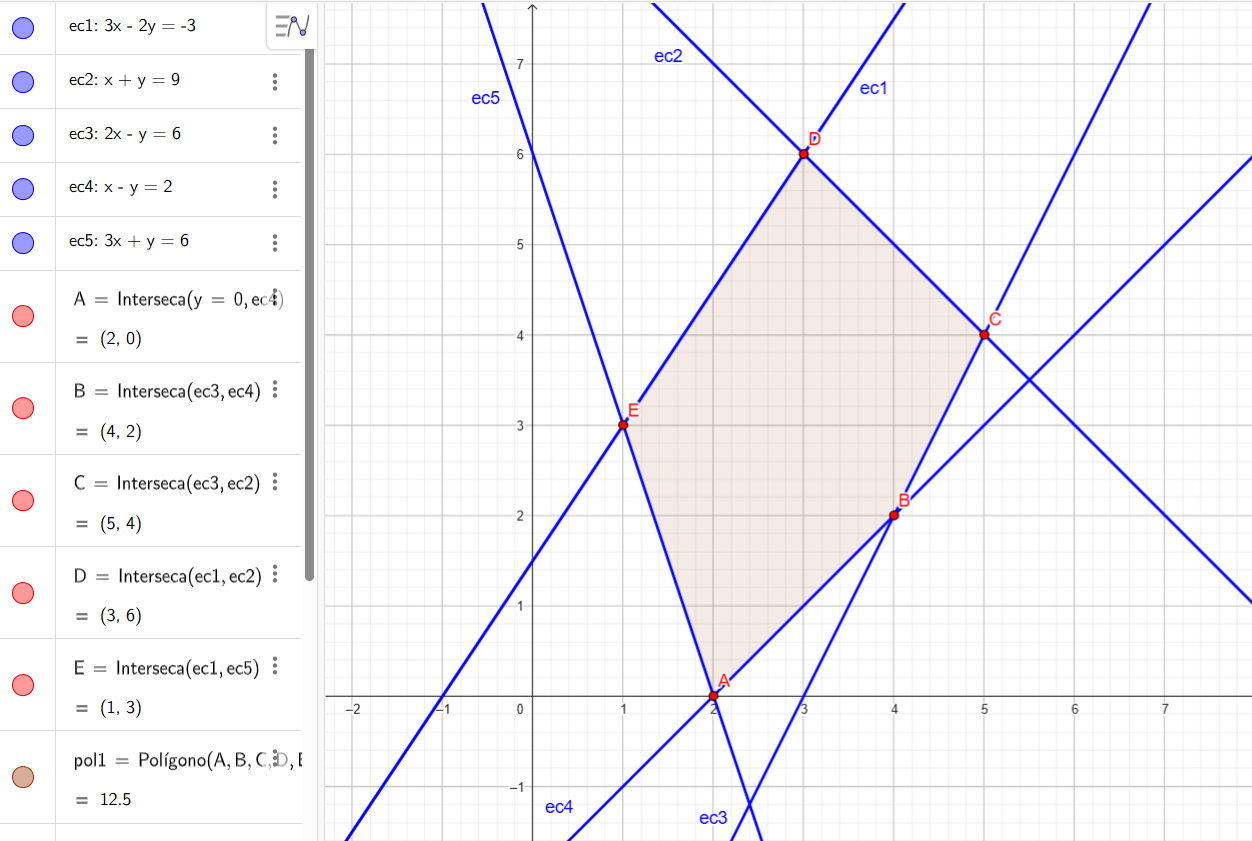
\includegraphics[width=\textwidth]{img/Ejercicio2.png}
\end{figure}
\begin{center}
    \begin{tabular}{|c|c|c|}
        \hline
        \textbf{Vertice ($x_1,x_2$)} & Z &  \\ \hline
        A(2, 0) & 10 & \\ \hline
        B(4, 2) & 24 & \\ \hline
        C(5, 4) & 33 & * \\ \hline
        D(3, 6) & 27 & \\ \hline
        E(1, 3) & 11 & \\ \hline
    \end{tabular}
\end{center}

\textbf{Soluci\'on \'Optima:}
\begin{align*}
    x_1 &= 5 \\ 
    x_2 &= 4 \\
    Z &= 33
\end{align*}

\newpage
\section*{Problema 3}

Considere el siguiente modelo lineal.
\begin{equation*}
    \begin{aligned}
        \text{Max} \quad & Z = 4x_1 + 3x_2 \\
        \text{s.a} \quad & 12x_1 + 14x_2 \leq 84 \quad \text{(Recurso 1)} \\
        & 3x_1 + 2x_2 \leq 18 \quad \text{(Recurso 2)} \\
        & x_2 \leq 4 \quad \text{(Recurso 3)} \\
        & x_1, x_2 \geq 0
    \end{aligned}
\end{equation*}

A continuaci\'on, se presenta una iteraci\'on intermedia del m\'etodo simplex para el problema anterior.
\begin{center}
    \begin{tabular}{|c|c|c|c|c|c|c|c|}
        \hline
        & & 4 & 3 & 0 & 0 & 0 & 0 \\ \hline
        $C_j$ & \textbf{V.B} & $x_1$ & $x_2$ & $s_1$ & $s_2$ & $s_3$ & RHS \\ \hline
        0 & $s_1$ & 0 & 6 & 1 & -4 & 0 & 12 \\
        4 & $x_1$ & 1 & 2/3 & 0 & 1/3 & 0 & 6 \\
        0 & $s_3$ & 0 & 1 & 0 & 0 & 1 & 4 \\ \hline
        & $Z_j$ & 4 & 8/3 & 0 & 4/3 & 0 & $\underline{24}$ \\ \hline
        & $C_j - Z_j$ & 0 & 1/3 & 0 & -4/3 & 0 & \\ \hline
    \end{tabular}
\end{center}

\begin{enumerate}
    \renewcommand{\labelenumi}{\alph{enumi})}
    \item ¿Es esta la iteraci\'on \'optima? Explique.
    
    \textbf{No es la iteraci\'on \'optima}, ya que el la fila $C_j - Z_j$ hay valores positivo, lo que indica que no se ha llegado a la soluci\'on \'optima.
    
    \item Si no es \'optima obtenga las siguientes iteraciones \textbf{a partir de esta} hasta alcanzar la soluci\'on \'optima.
    \begin{equation*}
        \colorbox{green!50}{$V_{in}$} = \text{columna Max} \{C_j-Z_j\} = X_{j^*} \Rightarrow V_{in} = x_2 : \frac{1}{3}
    \end{equation*}

    \begin{align*}
        s_1: \frac{12}{6} = 2 \qquad x_1: \frac{6}{2/3} = 9 \qquad s_3: \frac{4}{1} = 4 \\
    \end{align*}
    \begin{equation*}
        \colorbox{red!50}{$V_{out}$} = \text{Min} \left\{ \frac{RHS}{coef_{ij^*}} \right\} = i^* \Rightarrow V_{out} = s_1 : 2
    \end{equation*}

    \begin{center}
        \begin{tabular}{|c|c|c|g|c|c|c|c|}
            \hline
            & & 4 & 3 & 0 & 0 & 0 & 0 \\ \hline
            $C_j$ & \textbf{V.B} & $x_1$ & $x_2$ & $s_1$ & $s_2$ & $s_3$ & RHS \\ \hline
            \rowcolor{red!50}0 & $s_1$ & 0 & 6 & 1 & -4 & 0 & 12 \\
            4 & $x_1$ & 1 & 2/3 & 0 & 1/3 & 0 & 6 \\
            0 & $s_3$ & 0 & 1 & 0 & 0 & 1 & 4 \\ \hline
            & $Z_j$ & 4 & 8/3 & 0 & 4/3 & 0 & $\underline{24}$ \\ \hline
            & $C_j - Z_j$ & 0 & 1/3 & 0 & -4/3 & 0 & \\ \hline
        \end{tabular}
    \end{center}
    \begin{center}
        $\text{Pivote} = a_{i^*j^*} = a_{12} = 6$
    \end{center}

    \newpage
    \begin{align*}
        x_2: \quad \textbf{N.E.P} &= \frac{\textbf{E.P.A}}{P} \Rightarrow \frac{\begin{array}{cccccc} 0 & 6 & 1 & -4 & 0 & 12 \end{array}}{6} \\
        &= \begin{array}{cccccc} 0 & 1 & \frac{1}{6} & -\frac{2}{3} & 0 & 2 \end{array}
    \end{align*}

    \begin{equation*}
        \begin{array}{ccccccc}
            x_1: & 1 & 2/3 & 0 & 1/3 & 0 & 6 \\
            -(2/3) & 0 & 1 & 1/6 & -2/3 & 0 & 2\\
            \\ \hline \\
            & 1 & 0 & -1/9 & 7/9 & 0 & 14/3
        \end{array}
    \end{equation*}
    
    \begin{equation*}
        \begin{array}{ccccccc}
            s_3: & 0 & 1 & 0 & 0 & 1 & 4 \\
            -(1) & 0 & 1 & 1/6 & -2/3 & 0 & 2\\
            \\ \hline \\
            & 0 & 0 & -1/6 & 2/3 & 1 & 2
        \end{array}
    \end{equation*}
    
    \begin{center}
        \begin{tabular}{|c|c|c|c|c|c|c|c|}
            \hline
            & & 4 & 3 & 0 & 0 & 0 & 0 \\ \hline
            $C_j$ & \textbf{V.B} & $x_1$ & $x_2$ & $s_1$ & $s_2$ & $s_3$ & RHS \\ \hline
            3 & $x_2$ & 0 & 1 & 1/6 & -2/3 & 0 & \cellcolor{Celeste!50}2 \\
            4 & $x_1$ & 1 & 0 & -1/9 & 7/9 & 0 & \cellcolor{Morado!50}14/3 \\
            0 & $s_3$ & 0 & 0 & -1/6 & 2/3 & 1 & \cellcolor{green!50}2 \\ \hline
            & $Z_j$ & 4 & 3 & \cellcolor{yellow}1/18 & \cellcolor{yellow}10/9 & \cellcolor{yellow}0 & \cellcolor{Salmon!50}$\underline{24.67}$ \\ \hline
            & $C_j - Z_j$ & 0 & 0 & -1/18 & -10/9 & 0 & \\ \hline
        \end{tabular}
    \end{center}

    \item En la tabla \'optima describa la soluci\'on, clasifique los recursos y indique los precios sombra de cada recurso.
    
    \textbf{Solución:}
    \begin{align*}
        x_1 &= \colorbox{Morado!50}{14/3} \\
        x_2 &= \colorbox{Celeste!50}{2} \\
        s_1 &= 0 \qquad &\textbf{Recurso escaso} \Rightarrow \textbf{Restricci\'on ACTIVA} \\
        s_2 &= 0 \qquad &\textbf{Recurso escaso} \Rightarrow \textbf{Restricci\'on ACTIVA} \\
        s_3 &= \colorbox{green!50}{2} \qquad &\textbf{Recurso abundante} \Rightarrow \textbf{Restricci\'on NO ACTIVA} \\
        Z &= \colorbox{Salmon!50}{24,67}
    \end{align*}
    \begin{equation*}
        \begin{aligned}
            \text{Max} \quad & Z = 4x_1 + 3x_2 \\
            \text{s.a} \quad & 12x_1 + 14x_2 \leq 84 \quad &\textbf{Restricci\'on ACTIVA} \\
            & 3x_1 + 2x_2 \leq 18 \quad &\textbf{Restricci\'on ACTIVA} \\
            & x_2 \leq 4 \quad &\textbf{Restricci\'on NO ACTIVA} \\
            & x_1, x_2 \geq 0
        \end{aligned}
    \end{equation*}

    \textbf{Precios Sombra:}
    \begin{align*}
        \begin{array}{ccc}
            s_1 \Rightarrow \colorbox{yellow}{1/18} & s_2 \Rightarrow \colorbox{yellow}{10/9} & s_3 \Rightarrow \colorbox{yellow}{0}
        \end{array}
    \end{align*}
\end{enumerate}

\newpage
\section*{Problema 4}
Una compa\~n\'ia de las instalaciones A, B y C suministran a los distribuidores D, E, F y G.
Las capacidades mensuales son 20, 30 y 45 unidades, respectivamente; los requerimientos mensuales de los distribuidores son 10, 15, 40 y 30 unidades, para los distribuidores D, E, F y G; los costos unitarios de env\'io son los siguientes:
\begin{center}
    \begin{tabular}{|c|cccc|}
        \hline
        & D & E & F & G \\ \hline
        A & 5 & 10 & 5 & 0 \\
        B & 5 & 9 & 5 & 10 \\
        C & 10 & 10 & 15 & 5 \\ \hline
    \end{tabular}
\end{center}

\begin{enumerate}
    \renewcommand{\labelenumi}{\alph{enumi})}
    \item Determinar una soluci\'on sub \'optima utilizando Regla Noroeste.
    \begin{center}
        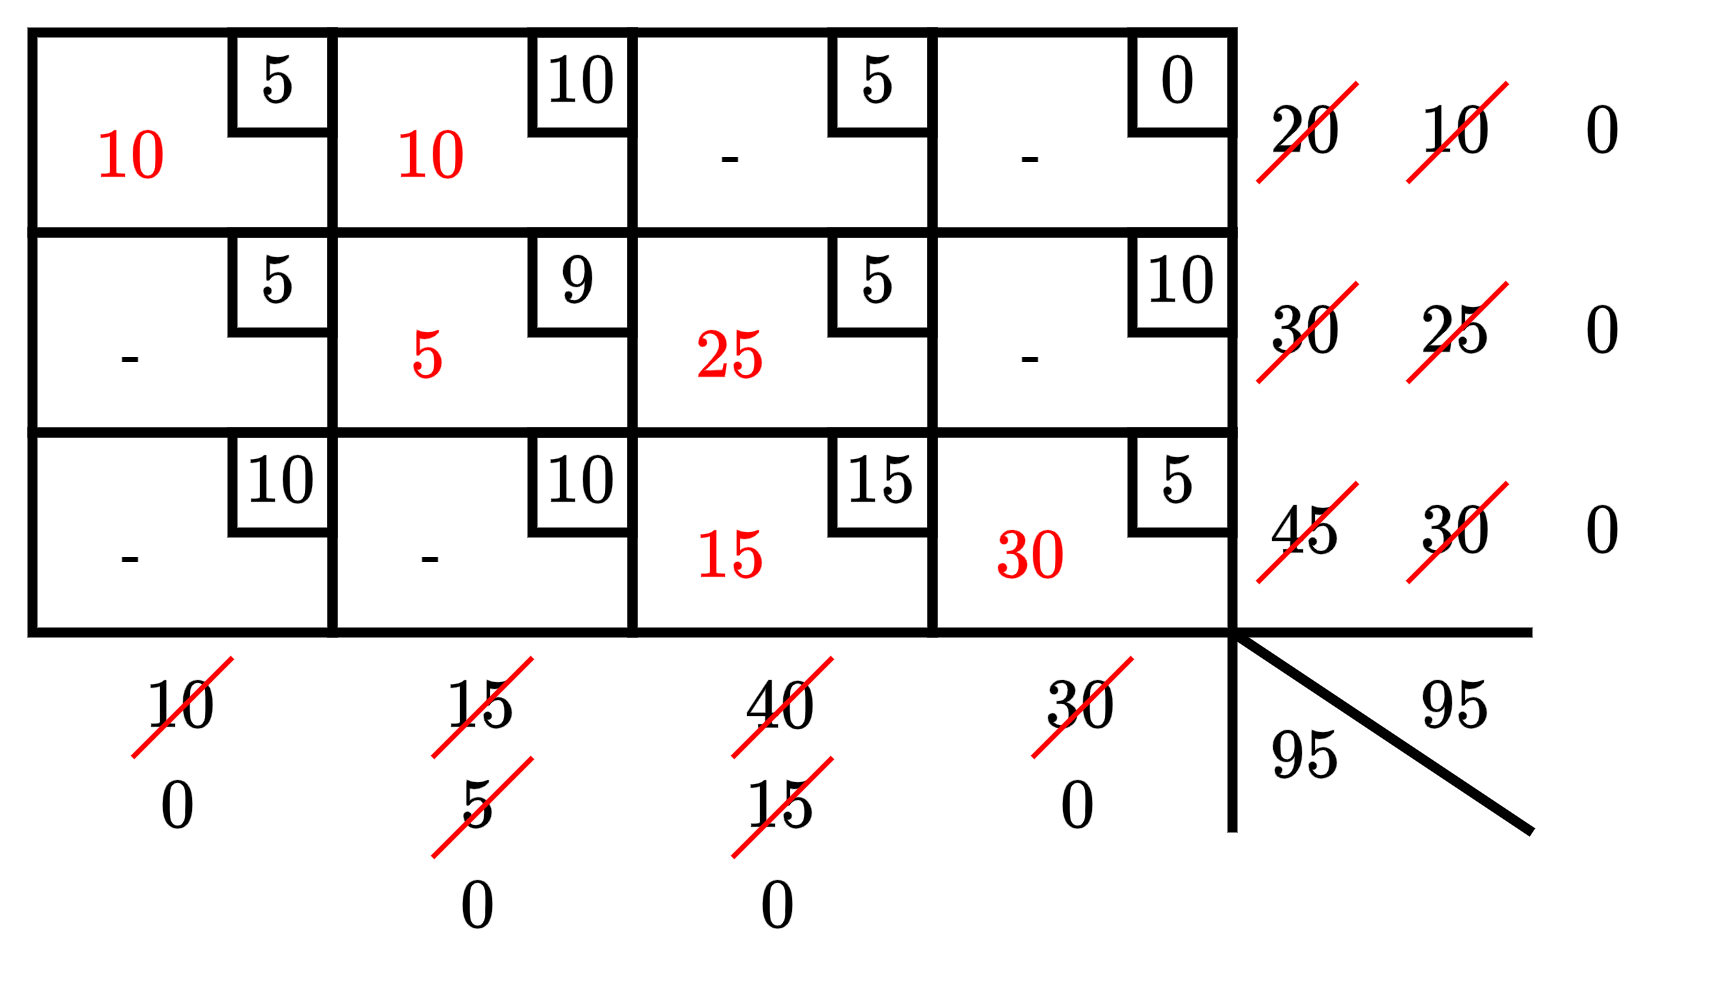
\includegraphics[width=0.6\textwidth]{diagram/Problema4-a.png}
    \end{center}

    \item ¿Cu\'anto se transporta por cada ruta?
    
    \begin{minipage}{0.6\textwidth}
        \begin{flushleft}
            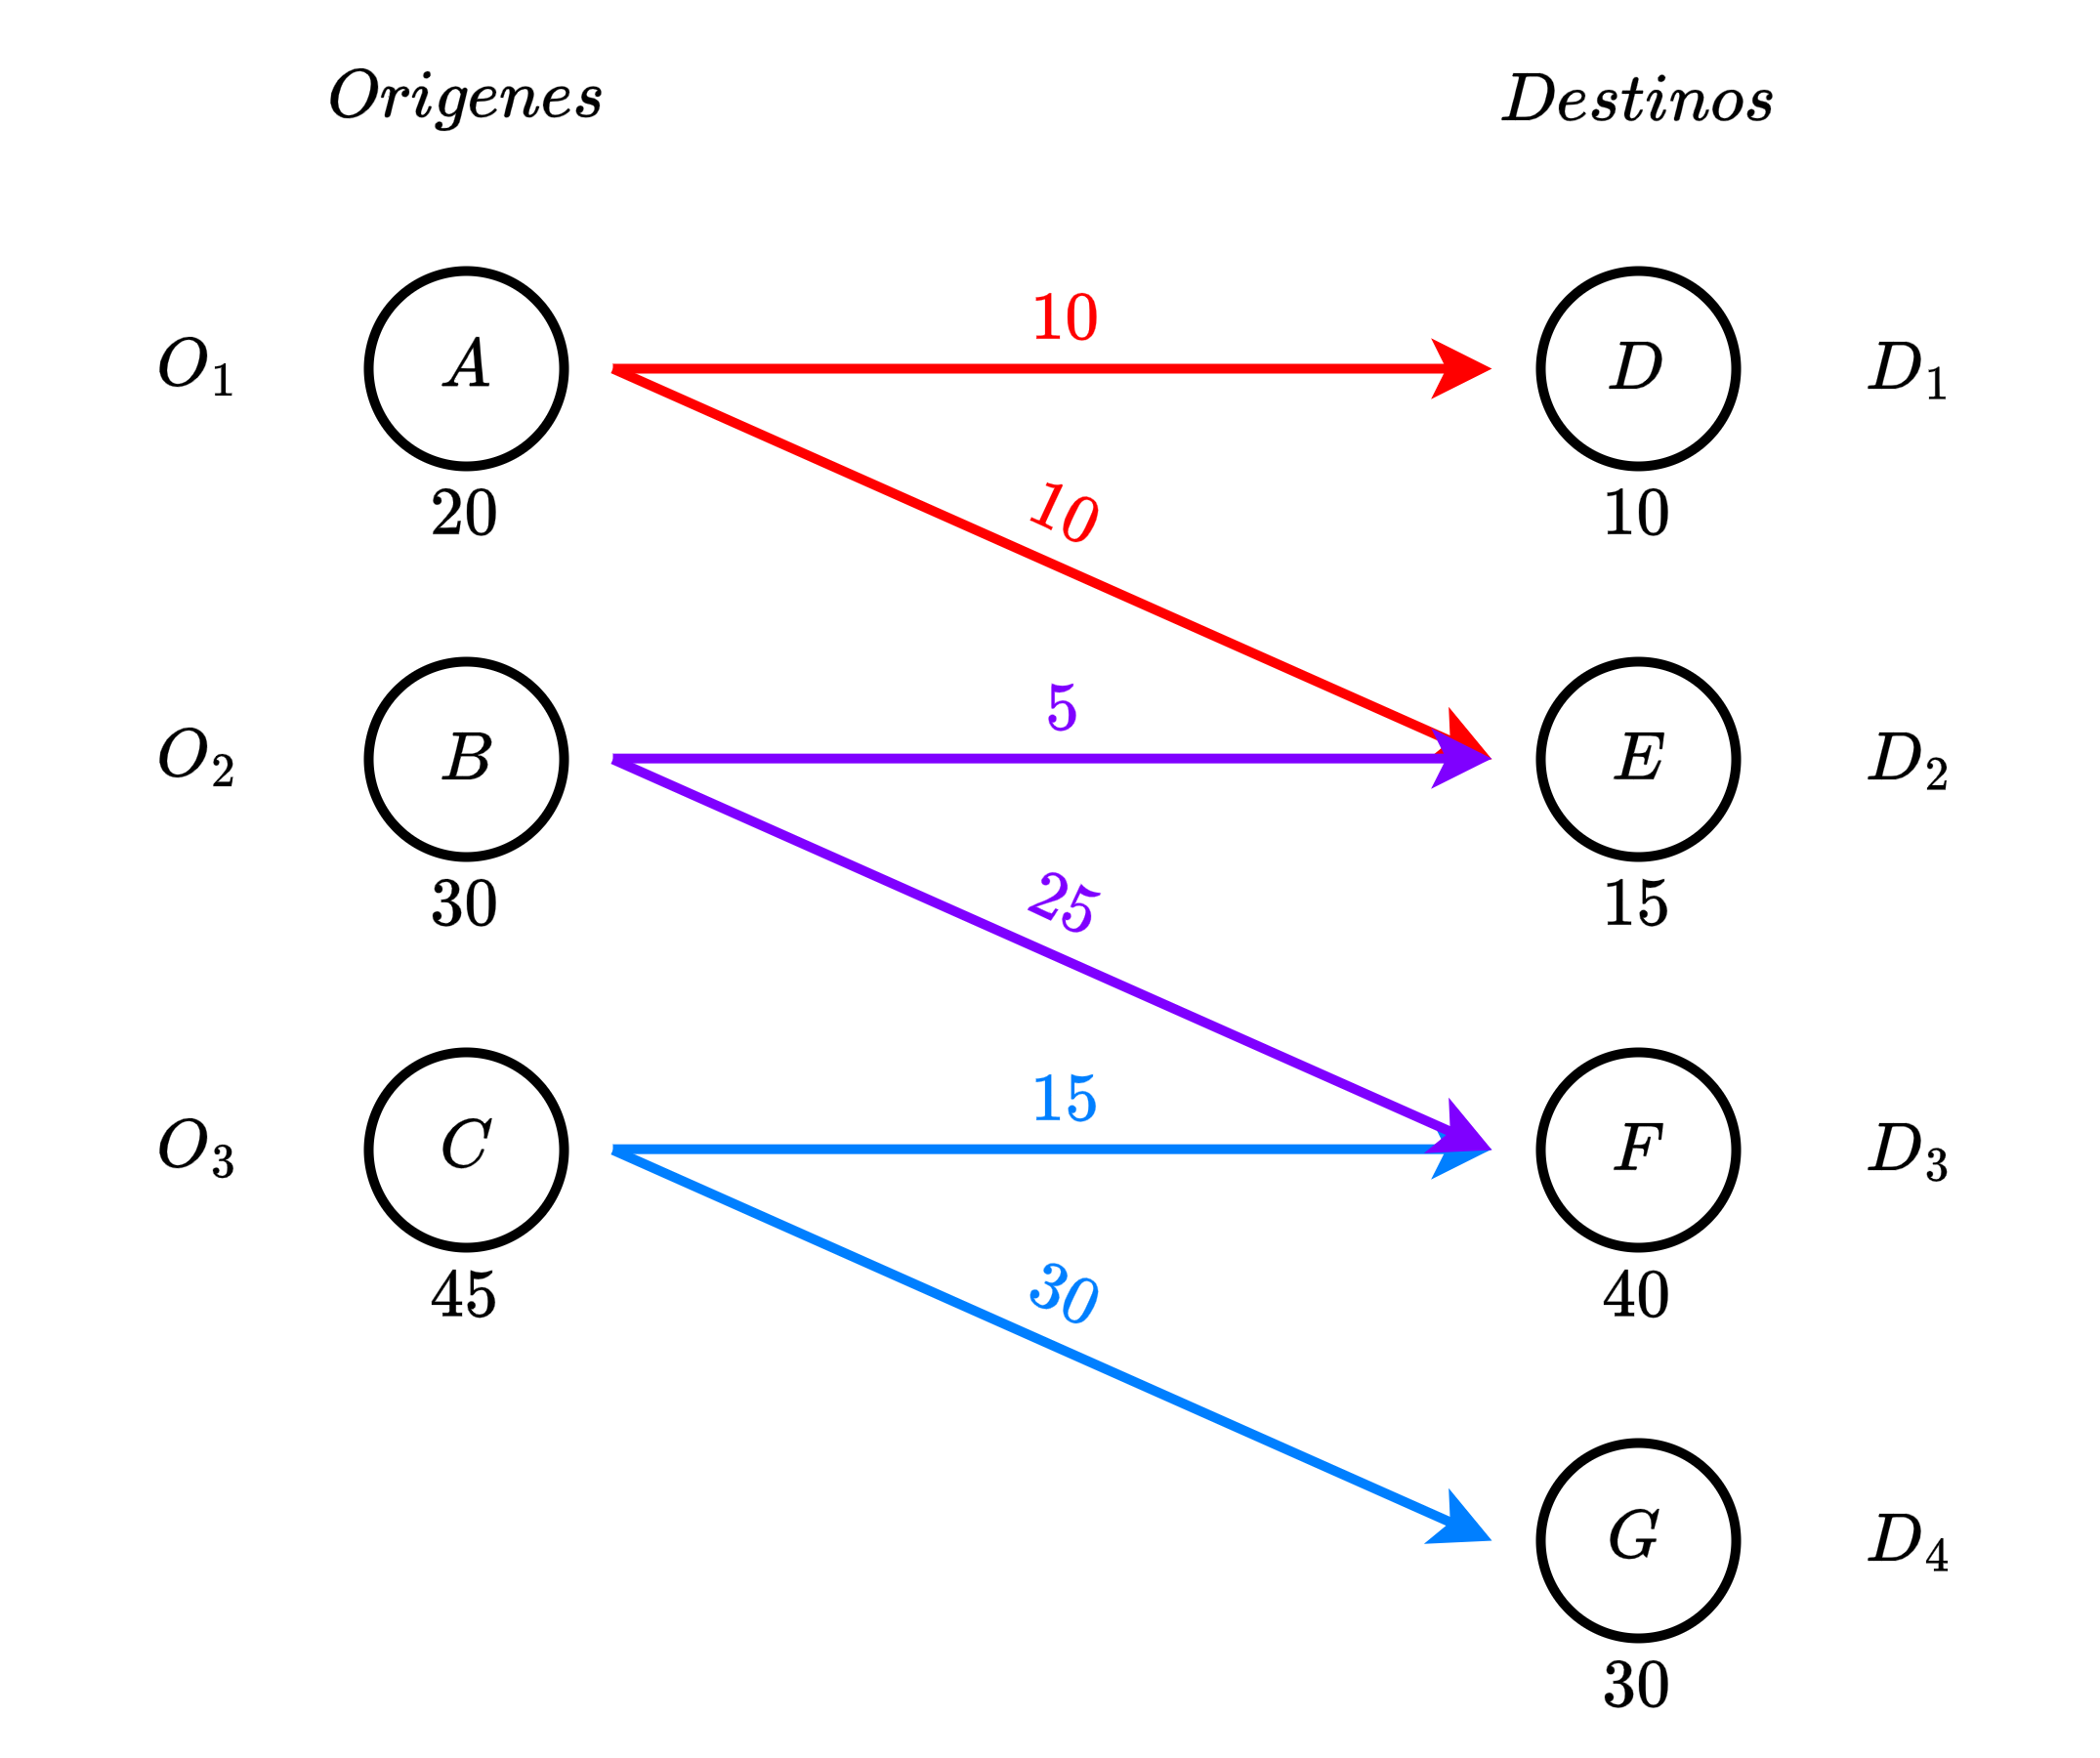
\includegraphics[width=0.9\textwidth]{diagram/Problema4-b.png}
        \end{flushleft}
    \end{minipage}
    \hfill
    \begin{minipage}{0.3\textwidth}
        \begin{itemize}
            \item De A a D: 10
            \item De A a E: 10
            \item De B a E: 5
            \item De B a F: 25
            \item De C a F: 15
            \item De C a G: 30
        \end{itemize}
    \end{minipage}

    $X_{11}=10$, $X_{12}=10$, $X_{22}=5$, $X_{23}=25$, $X_{33}=15$, $X_{34}=30$
    \item ¿Cu\'al es el costo total de transporte que da esta soluci\'on?
    \begin{align*}
        Z &= 10 \cdot 5 + 10 \cdot 10 + 5 \cdot 9 + 25 \cdot 5 + 15 \cdot 15 + 30 \cdot 5 \\
        &= 50 + 100 + 45 + 125 + 225 + 150 \\
        &= 695
    \end{align*}
    
    \newpage
    \item ¿Es \'optima la soluci\'on Noroeste? Explique.
    
    No es \'optima, pues utilizando el criterio de \'optimalidad, se dice:
    
    \begin{itemize}
        \item Si todos los costos reducidos son $\geq 0$, entonces hemos llegado a la soluci\'on \'optima.
    \end{itemize}

    Al calcular los costos reducidos, se obtiene lo siguiente:
    \begin{center}
        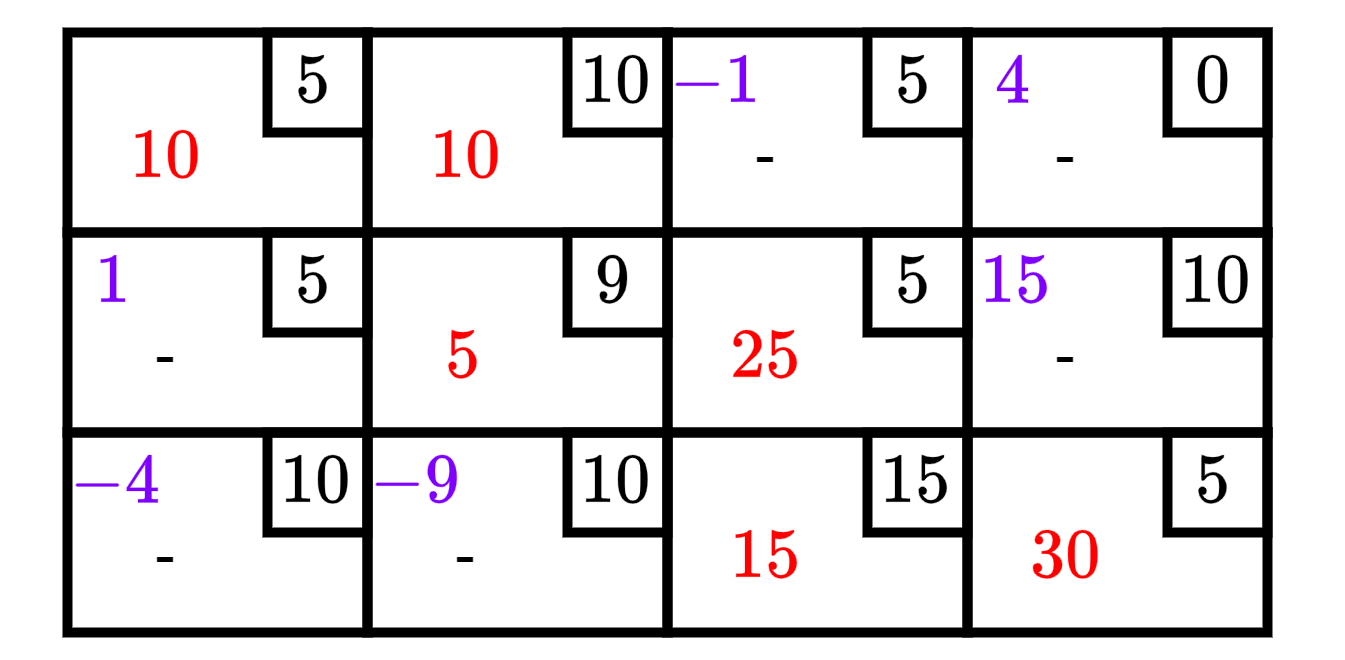
\includegraphics[width=0.6\textwidth]{diagram/Problema4-d.png}
    \end{center}

    Podemos observar que las casillas $x_{13}, x_{31}, x_{32}$ tienen valores negativos, por lo que no hemos llegado a la soluci\'on \'optima.

    \item Si no es \'optima realice una iteraci\'on adicional e indique cuanto mejora la nueva soluci\'on.
    \begin{center}
        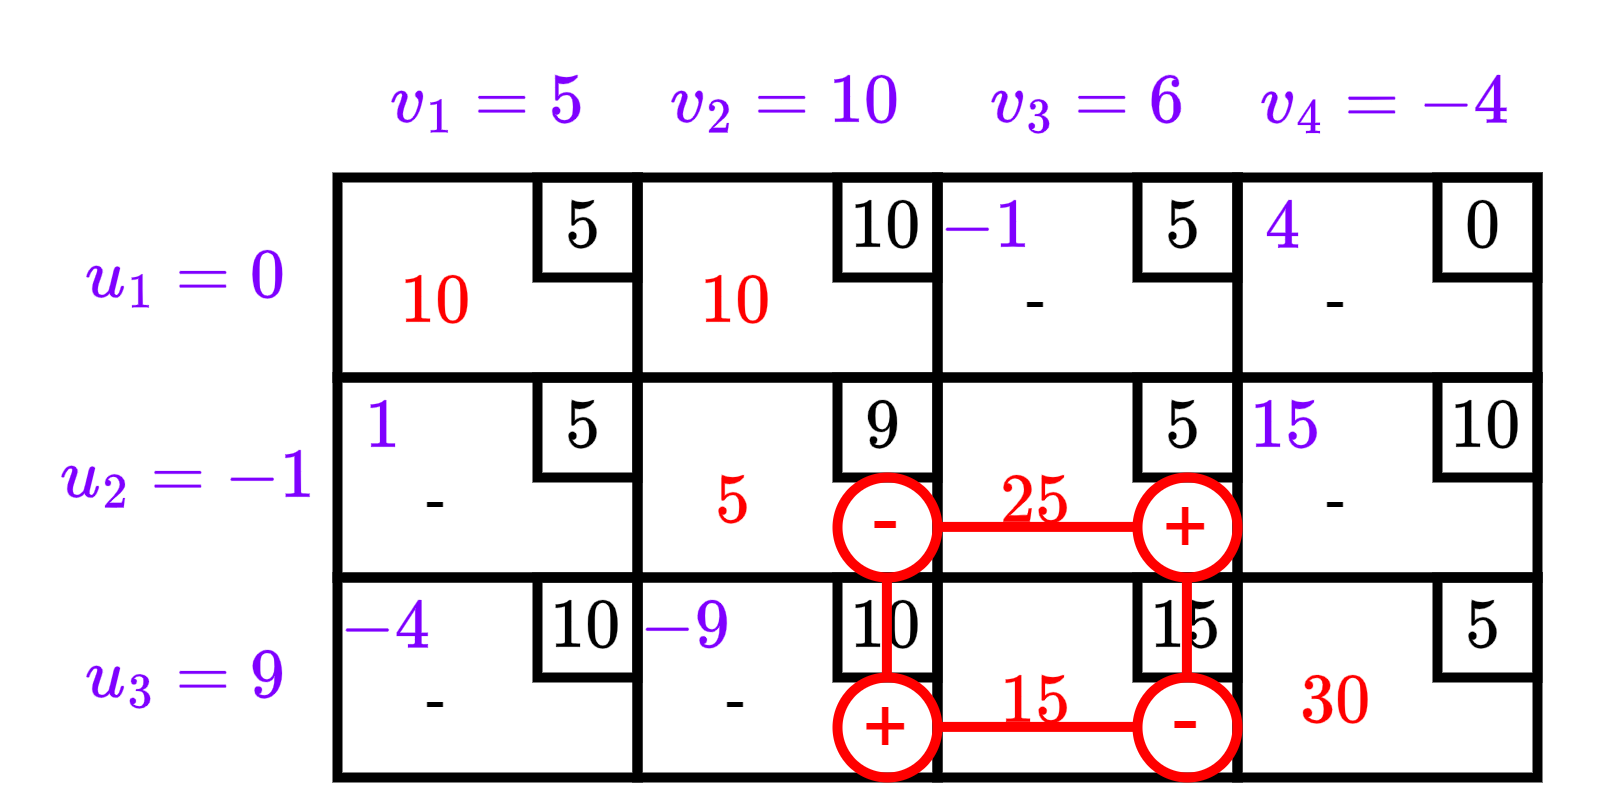
\includegraphics[width=0.7\textwidth]{diagram/Problema4-e-1.png}
    \end{center}
    \begin{center}
        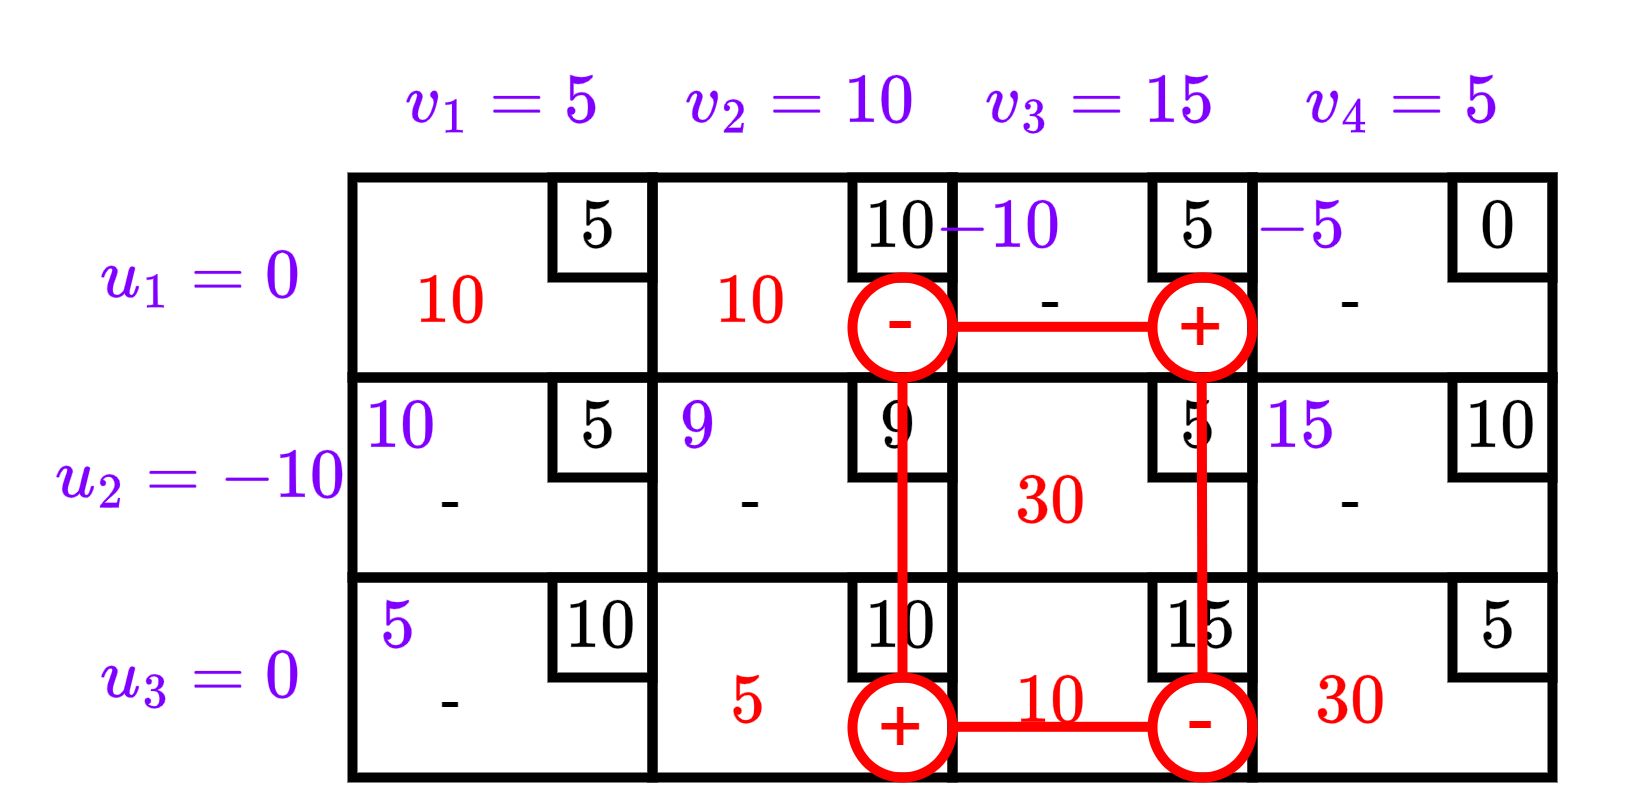
\includegraphics[width=0.7\textwidth]{diagram/Problema4-e-2.png}
    \end{center}
    \begin{center}
        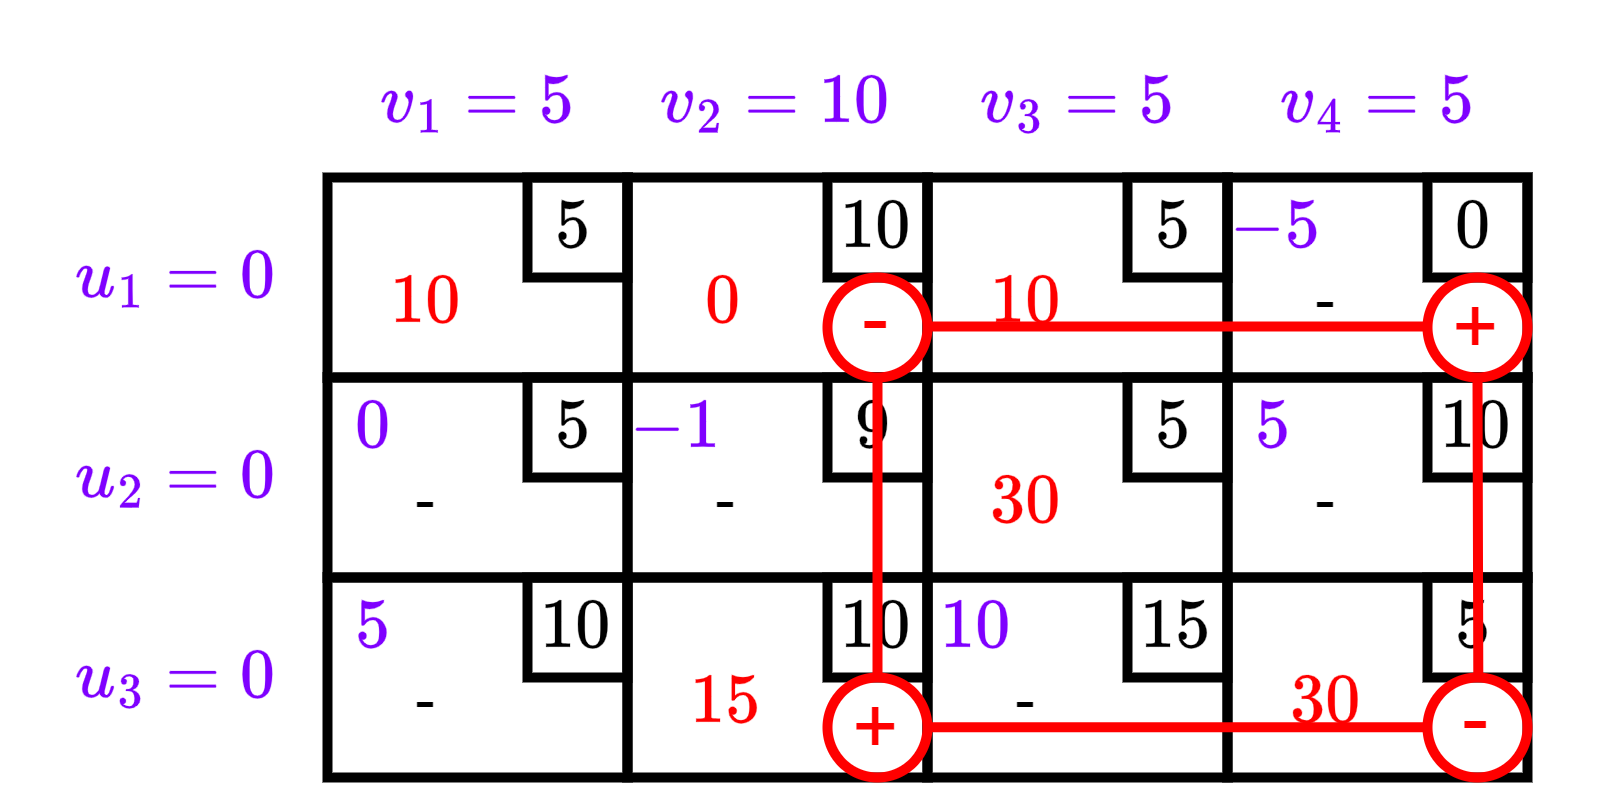
\includegraphics[width=0.7\textwidth]{diagram/Problema4-e-3.png}
    \end{center}
    \begin{center}
        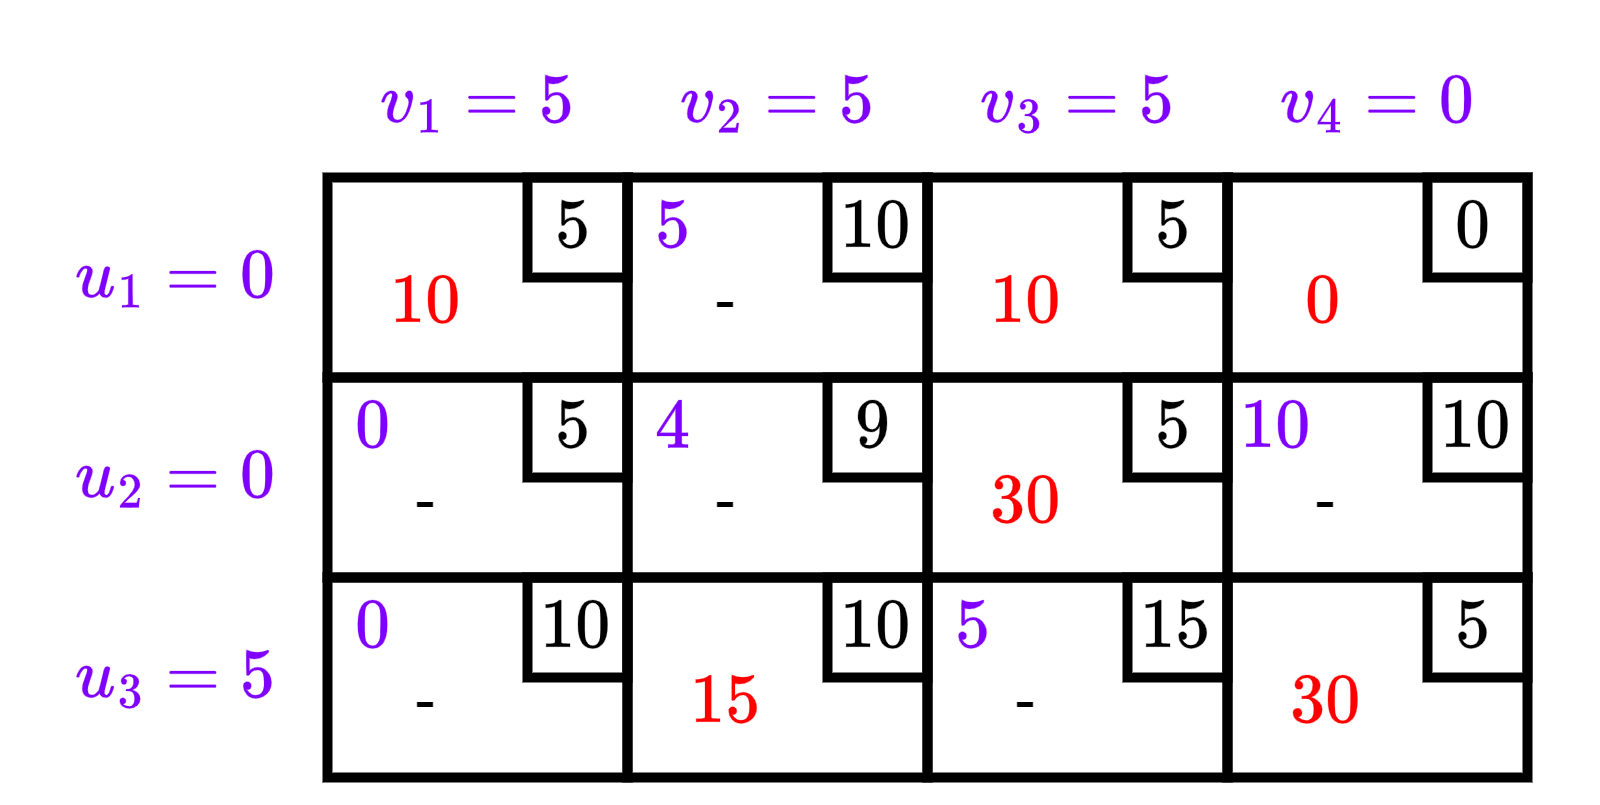
\includegraphics[width=0.7\textwidth]{diagram/Problema4-e-4.png}
    \end{center}

    Como todos los costos reducidos son $\geq 0$, entonces hemos llegado a la soluci\'on \'optima.
    \begin{align*}
        Z &= 10 \cdot 5 + 10 \cdot 5 + 0 \cdot 0 + 30 \cdot 5 + 15 \cdot 10 + 30 \cdot 5 \\
        &= 50 + 50 + 0 + 150 + 150 + 150 \\
        &= 550
    \end{align*}
\end{enumerate}

\newpage
\section*{Problema 5}
Una empresa desea asignar 5 operaciones ($O_i$) a 5 m\'aquinas ($M_j$). Los costos de las posibles asignaciones aparecen en la siguiente tabla.
\begin{center}
    \begin{tabular}{|c|ccccc|}
        \hline
        & $M_1$ & $M_2$ & $M_3$ & $M_4$ & $M_5$ \\ \hline
        $O_1$ & 15 & 16 & \cellcolor{orange}15 & 14 & 13 \\
        $O_2$ & 36 & 35 & 34 & 30 & \cellcolor{orange}29 \\
        $O_3$ & 26 & 25 & 29 & \cellcolor{orange}22 & 28 \\
        $O_4$ & 20 & \cellcolor{orange}16 & 25 & 23 & 15 \\
        $O_5$ & \cellcolor{orange}26 & 28 & 29 & 24 & 25 \\ \hline
    \end{tabular}
\end{center}

Con estos datos y aplicando el m\'etodo h\'ungaro, determinar la mejor asignaci\'on posible y el costo resultante.

\begin{minipage}{0.5\textwidth}
    \begin{itemize}
        \item \textbf{Paso 1:} Restar el menor valor de cada fila a todos los elementos de la fila.
        \begin{center}
            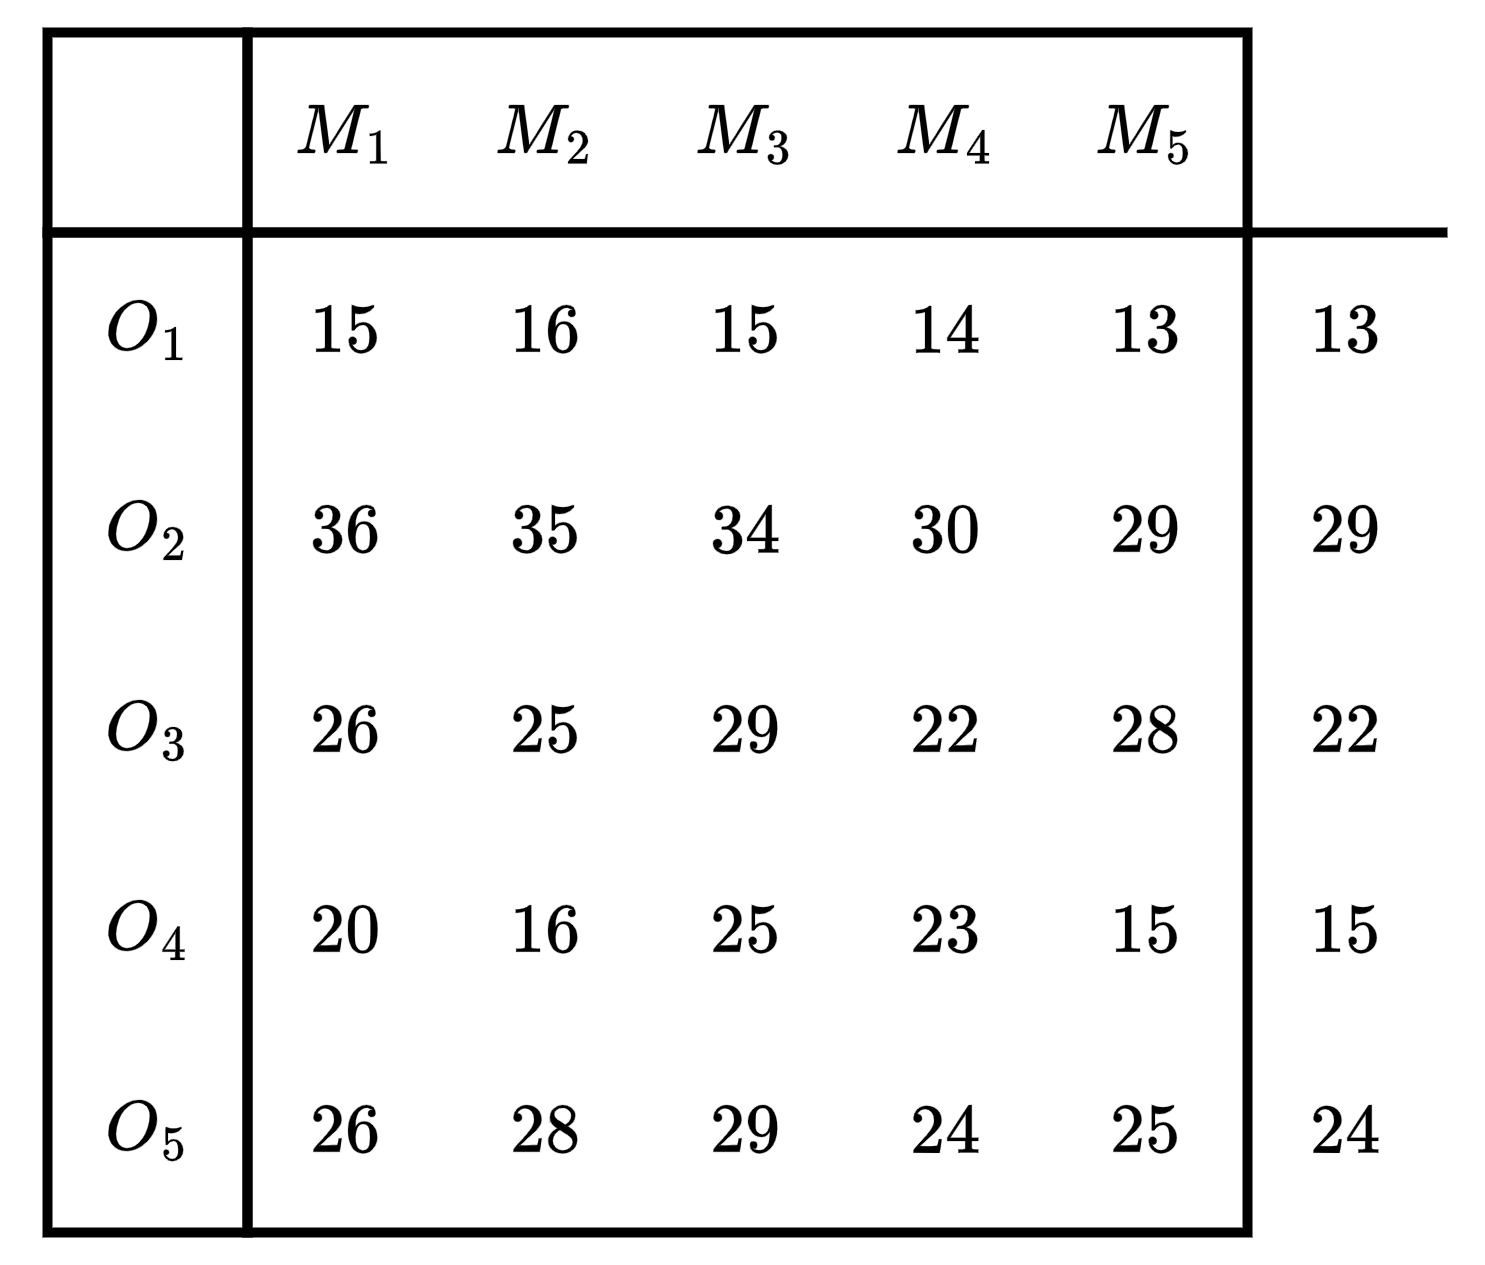
\includegraphics[width=0.7\textwidth]{diagram/Problema5-1.png}
        \end{center}

        \item \textbf{Paso 2:} Restar el menor valor de cada columna a todos los elementos de la columna.
        \begin{center}
            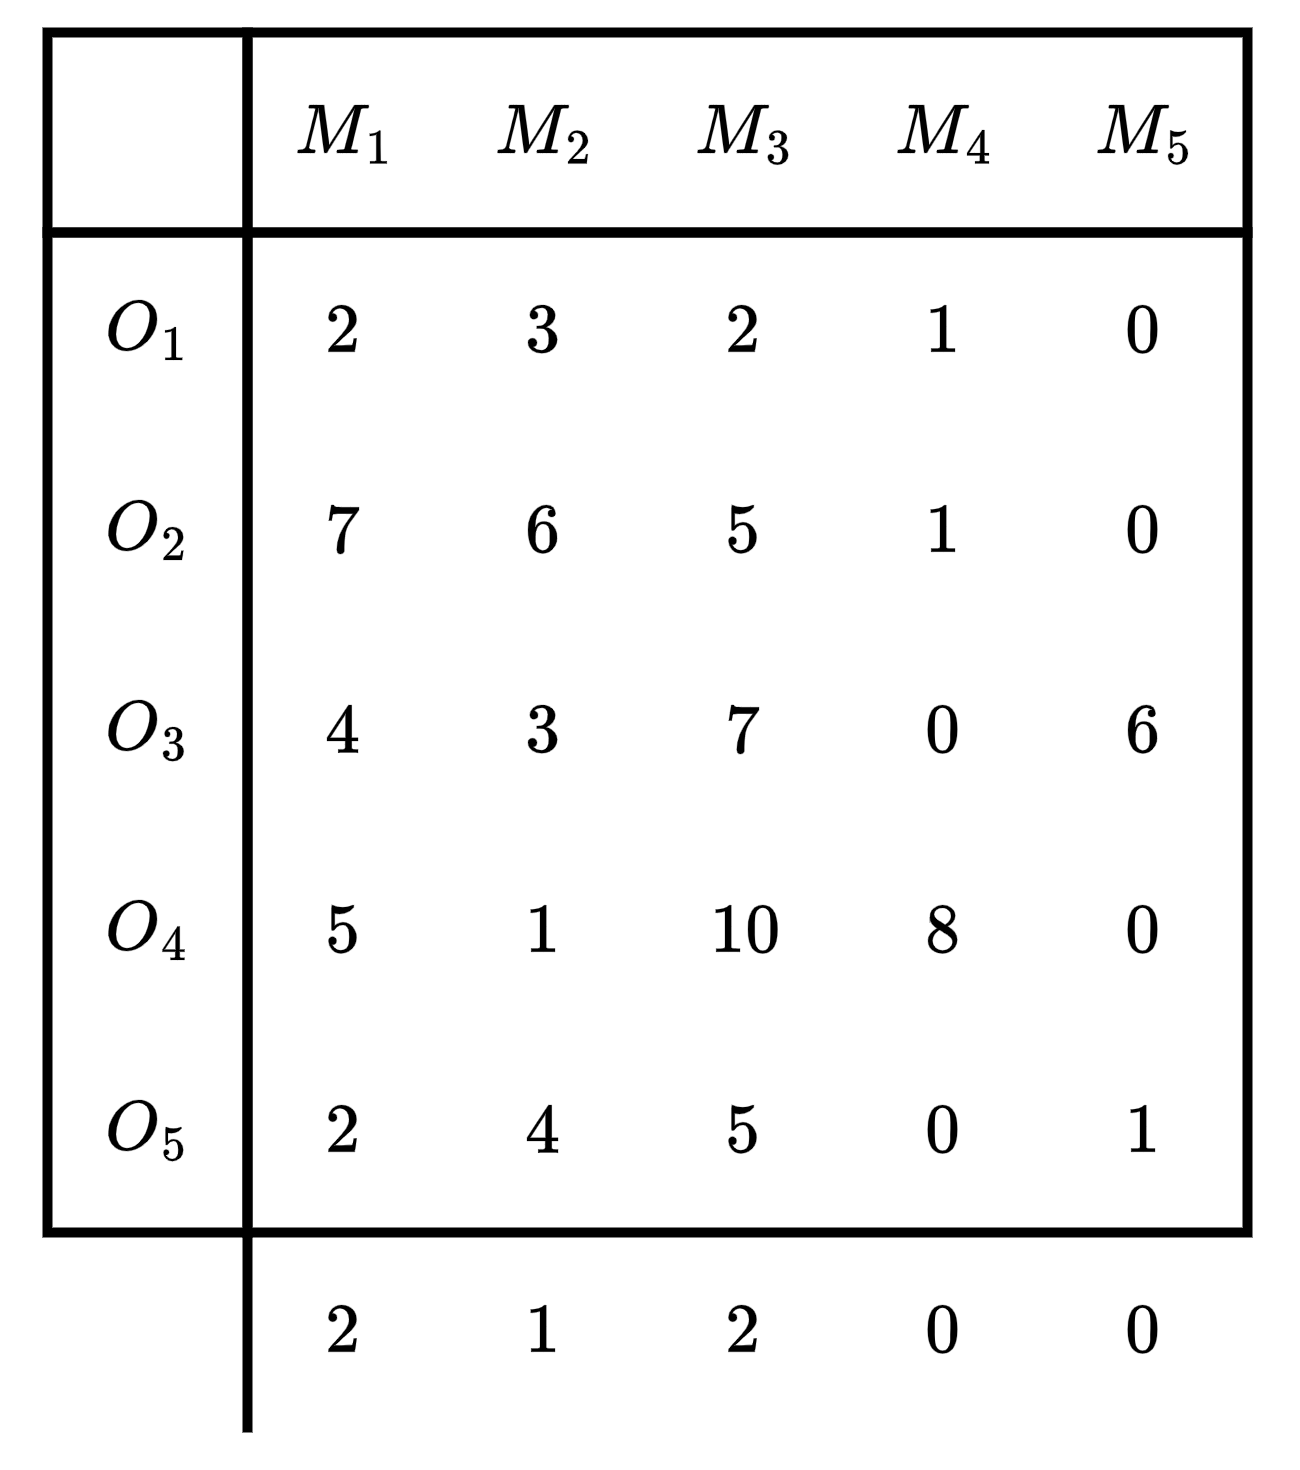
\includegraphics[width=0.6\textwidth]{diagram/Problema5-2.png}
        \end{center}    
    \end{itemize}
\end{minipage}
\hfill
\begin{minipage}{0.4\textwidth}
    \begin{itemize}
        \item \textbf{Paso 3:} Elegir los ceros de la matriz, eligiendo desde el m\'as restrictivo (con menos ceros) hasta dejar un solo cero en cada fila y columna.
    \end{itemize}
    \begin{center}
        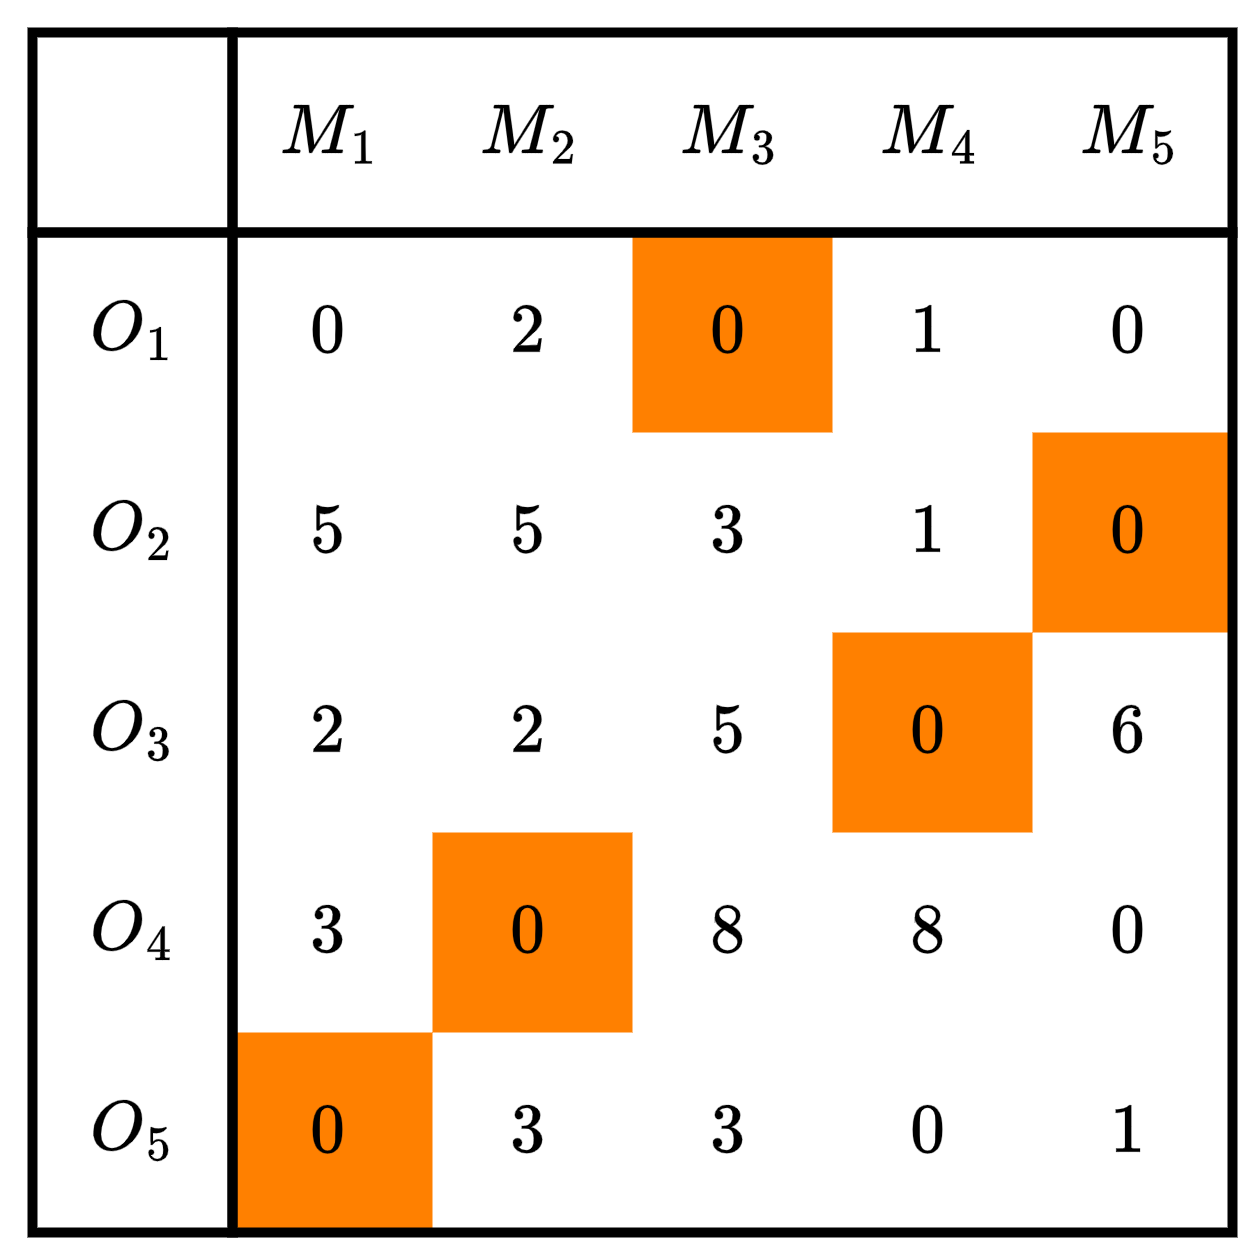
\includegraphics[width=0.7\textwidth]{diagram/Problema5-3.png}
    \end{center}
    \textbf{Soluci\'on \'optima:}
    \begin{center}
        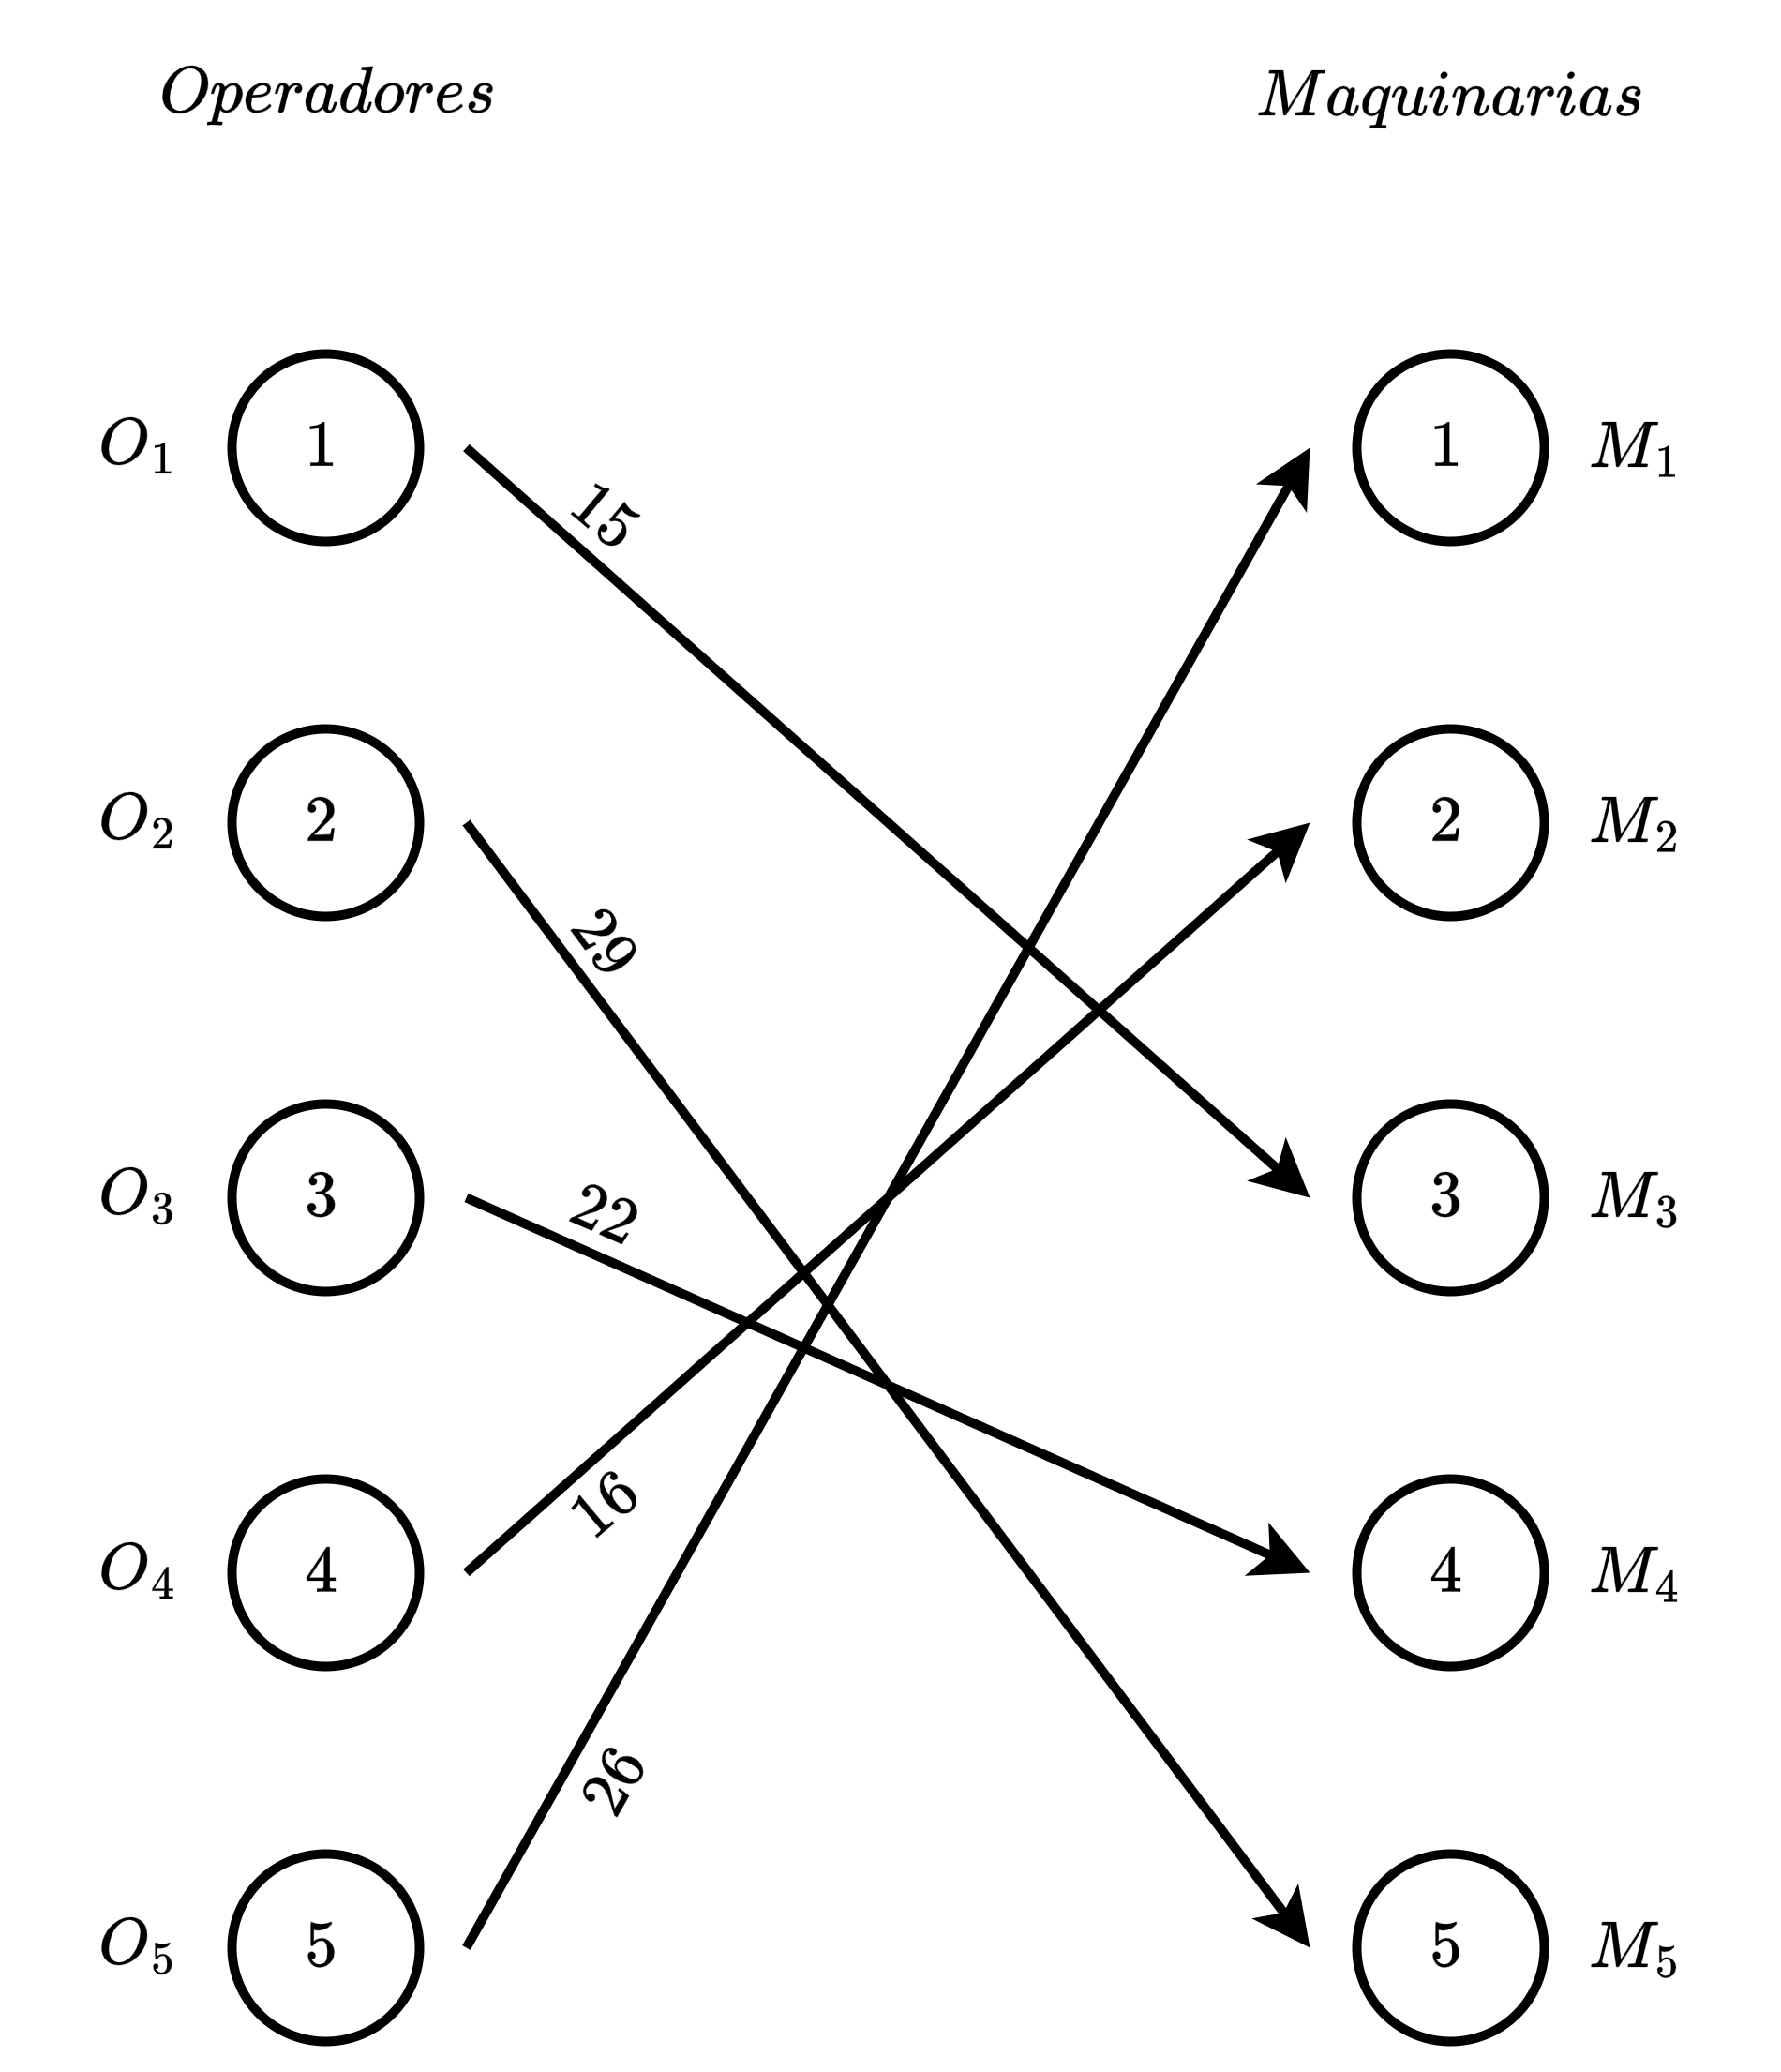
\includegraphics[width=0.6\textwidth]{diagram/Problema5-4.png}
    \end{center}
\end{minipage}
\begin{align*}
    Z &= 15 + 29 + 22 + 16 + 26 \\
    &= 108
\end{align*}

\end{document}